\section{Scale and reliability}

The scale question is practical measurement advantage over
the response-function measurement null set out in the secondary-data design.
Bard et al.'s case for magnitude estimation included scale resolution,
fine-grained distinctions, naive-participant use, and replication across groups
\citep[32]{BardEtAl1996}. The safer target is that source-grounded claim,
together with the stronger reading of magnitude estimation that took hold in
parts of the later methodology literature.

Later method-comparison data give the paper a sharper question: does magnitude
estimation recover item differences, participant agreement, or theoretically
relevant decisions that simpler tasks lose, and in particular does it recover
graded distinctions that bounded scales compress at the extremes?

\textcite{sprouse2013} compare formal judgment tasks with informal published
judgments, giving evidence about convergence between magnitude estimation,
Likert ratings, and forced choice. The public rows from that study can support a
bounded reanalysis of item-level agreement and decision consequences within
the approved reuse boundary. \textcite{LangsfordEtAl2018} add a reliability and
response-bias target by comparing Likert, magnitude estimation, forced choice,
and Thurstonian models. Without their raw rows, Langsford can support the
synthesis of published reliability findings but not a new participant-level
response-style or test-retest model.

The reanalysis inherits the unit-of-analysis charter fixed in the secondary-data
design rather than reopening it. The same primary and sensitivity
representations carry over, so the claims stay traceable to fixed units of
analysis instead of to whichever representation later proves most convenient.

The primary comparison weighs methods on resolution, prediction, decision
consequences, and convergence, prioritizing consequences for the linguistic
contrast. Resolution is the criterion Bard's claim lives on: whether magnitude
estimation recovers graded item differences that bounded scales compress at
ceiling or floor, or a measurement dimension that survives the dimensionality
check. Reliability is a distinct property, not a proxy for it;
\textcite{LangsfordEtAl2018} report magnitude estimation as less reliable, which
doesn't by itself settle resolution.

For this paper, a practical magnitude-estimation advantage would have to change
an inferential decision. A summary-statistic improvement alone wouldn't count.
An advantage would count if magnitude estimation recovered a good-vs-bad contrast that
bounded methods missed, showed its largest extra spread exactly where bounded
scales compressed the response, carried a stable method-specific dimension
across scoring choices, or reduced sign-error or exaggeration risk for a named
contrast under a design analysis. A larger correlation, by itself, wouldn't
settle the question.

The reanalysis of both comparison datasets gives a narrow answer. Magnitude
estimation and the bounded methods share a strong aggregate item-level signal. Raw Likert means
also show the expected bounded response-function curvature relative to magnitude
estimation. That curvature is the pattern Bard's scale argument makes visible,
but the endpoint and pair-level diagnostics don't show a systematic practical
distinction preserved only by magnitude estimation.

Figure~\ref{fig:response-functions} makes the common signal and bounded
curvature visible. The linear fit tracks the centre of each cloud but runs past
the Likert scale's upper boundary, while the bounded fit turns towards that
boundary. That pattern is why the analysis allows method-specific response functions
before asking whether magnitude estimation preserves a further practical
distinction.

\begin{figure}[H]
\centering
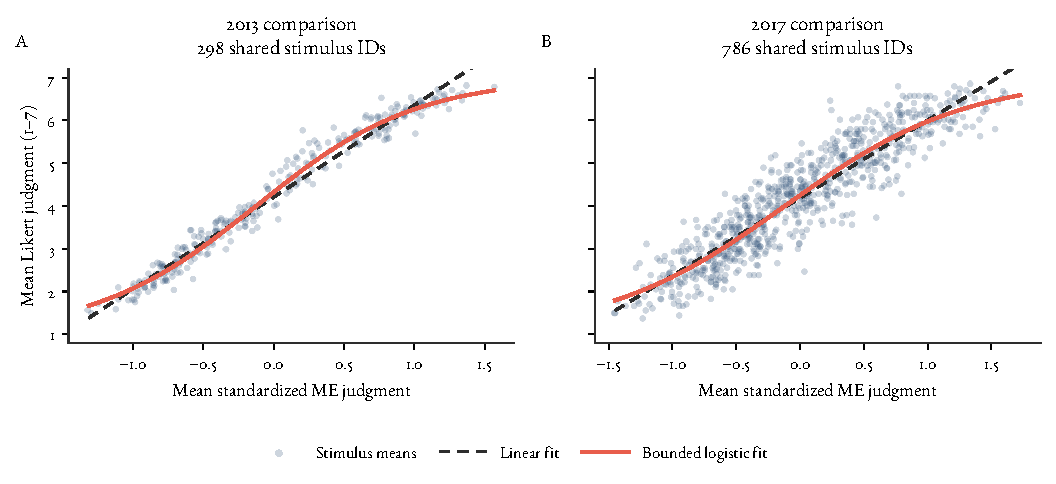
\includegraphics[width=\linewidth]{figures/response-functions.pdf}
\caption{Aggregate response functions in the public comparison data from
Sprouse, Sch\"utze, and Almeida (2013) (A) and Sprouse and Almeida (2017) (B).
Each point averages participant judgments for one stimulus identifier shared by
the magnitude-estimation and Likert files. The 2013 files call these identifiers
\enquote{conditions} (298 points); the 2017 files call them \enquote{items} (786
points). The two labels reproduce the source-file nomenclature. The dashed line
is a linear fit and the solid line is a 1--7 bounded logistic fit. Magnitude
estimation is an unbounded diagnostic axis here, not the assumed true latent
acceptability scale.}
\label{fig:response-functions}
\end{figure}

The dimensionality result is deliberately modest: a first-pass aggregate
check of the item and contrast matrices, used to ask whether a clear
multidimensional rescue for magnitude estimation appears in the available
aggregate summaries. It doesn't replace a full participant-level factor model,
which would require a broader row-level evidence base than this paper has.

The rows in Table~\ref{tab:sprouse-diagnostics} come from the approved pipeline
documented in \texttt{analysis/README.md}: item-signal, dimensionality,
response-function, pair-robustness, and aggregate sensitivity scripts. The
reported \(n\) values are aggregate condition, item, or pair units, not
participant-level rows. A 95\% percentile bootstrap over those same aggregate
units gives intervals that leave the interpretation unchanged: ME--Likert
correlations remain high for 2013 conditions [.983, .989], 2013 pairs [.950,
.974], 2017 items [.915, .934], and 2017 pairs [.917, .965], and pair-level
bounded-predictor \Rsq{} remains high for 2013 [.900, .946] and 2017
[.862, .941].

\begin{table}[H]
\centering
\small
\renewcommand{\arraystretch}{1.08}
\begin{tabular}{@{}>{\raggedright\arraybackslash}p{0.23\linewidth}>{\raggedright\arraybackslash}p{0.34\linewidth}>{\raggedright\arraybackslash}p{0.34\linewidth}@{}}
\toprule
Diagnostic & 2013 study & 2017 study \\
\midrule
ME--Likert convergence & Conditions \(n=298\), \(r=.986\); pairs \(n=150\), \(r=.963\) & Items \(n=786\), \(r=.925\); pairs \(n=50\), \(r=.944\) \\ \addlinespace[2pt]
First-pass dimensionality check & Pairs \(n=150\): first component 89.4\%; second eigenvalue below parallel-analysis threshold & Items \(n=786\), pairs \(n=50\): first components 80.6\% and 85.9\%; second eigenvalues below thresholds \\ \addlinespace[2pt]
Bounded response function & Conditions \(n=298\): bounded logistic improves over linear; endpoint ME SDs .142 and .175 versus middle .313 & Items \(n=786\): bounded logistic improves over linear; endpoint ME SDs .249 and .321 versus middle .349 \\ \addlinespace[2pt]
Pair robustness & Pairs \(n=150\): bounded predictors \Rsq{} = .926; no ME top-quartile pair falls in the bounded bottom half & Pairs \(n=50\): bounded predictors \Rsq{} = .901; no ME top-quartile pair falls in the bounded bottom half \\
\bottomrule
\end{tabular}
\caption{Primary diagnostics from the comparison data accompanying Sprouse,
Sch\"utze, and Almeida (2013) and Sprouse and Almeida (2017) for Bard's
resolution claim. ME = magnitude estimation. The dimensionality row is an
aggregate first-pass check,
and the response-function rows use magnitude estimation as an unbounded
diagnostic axis rather than the true latent acceptability scale.}
\label{tab:sprouse-diagnostics}
\end{table}

Table~\ref{tab:sprouse-diagnostics} separates three facts. First, the
aggregate matrices provide no obvious multidimensional rescue for magnitude
estimation. Second, the Likert scale behaves like a bounded response function,
so a fair null should allow compression. Third, the available contrasts
don't show the further pattern that would make magnitude estimation
practically superior: endpoint regions aren't where magnitude estimation
spreads out most, and good-vs-bad pairs ranked highly by magnitude estimation
are also ranked highly by bounded methods.

The explicitly post-outcome multiverse asks whether that interpretation survives
defensible scoring and modelling choices. It varies three ME scores, three
Likert scores, endpoint definitions and spread statistics, raw- and rank-scale
prediction, and forced-choice or yes/no adjudication. None of its endpoint,
incremental-prediction, or decision-adjudication families meets the frozen
family-level criterion in either dataset.

The disaggregated result contains one useful qualification. Both endpoint ratios
exceed one in 3 of 27 specifications for 2013 and 6 of 27 for 2017; only one 2017
specification also clears the practical and permutation criteria. ME adds at
least .02 cross-validated \Rsq{} beyond Likert in 0 of 36 prediction
specifications for 2013 and 4 of 36 for 2017. Those four are rank-scale models
of forced choice (\deltaRsq{} = .025--.049); the increment doesn't generalize
to 2017 yes/no judgments or to raw-scale mappings. ME and Likert disagree on
the contrast sign for only 3 of 150 pairs in 2013 and 1 of 50 in 2017, too few
to clear the decision criterion. The localized 2017 result makes a blanket
no-information claim too strong for those specifications, but it doesn't
establish a systematic practical advantage.

Figure~\ref{fig:multiverse-landscape} shows why the qualification matters
without changing the family-level conclusion. The isolated endpoint result and
four prediction increments sit inside distributions dominated by smaller or
negative effects, while actual ME--Likert contrast-sign disagreements remain
rare.

\begin{figure}[H]
\centering
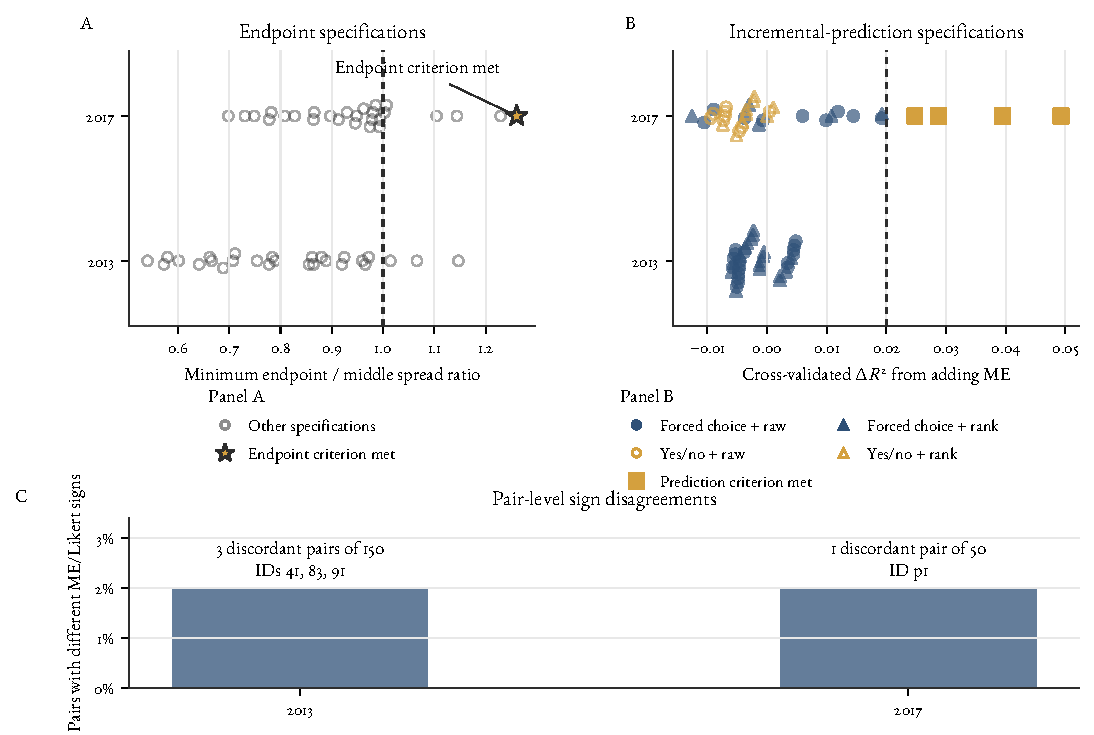
\includegraphics[width=\linewidth]{figures/multiverse-landscape.pdf}
\caption{The explicitly post-outcome multiverse. Panel A shows all 54 admissible
endpoint specifications; the dashed line marks equal minimum endpoint and
middle spread. The golden star is the sole specification in which both endpoint
ratios reach 1.25 and the permutation probability is below .05. Panel B shows
all 72 incremental-prediction specifications. Filled blue markers denote a
forced-choice target and open golden markers a yes/no target; circles denote
raw-scale mappings and triangles rank-scale mappings. Solid golden squares mark
the four specifications meeting the prediction criterion: \deltaRsq{} from
adding ME is at least .02 and exceeds the corresponding increment from adding
Likert. The dashed line marks the .02 threshold. Symmetric vertical stacking
separates nearby specifications; vertical position within a study row has no
substantive meaning. Panel C shows the proportion of pairs on which ME and
Likert disagree about the contrast sign; it uses pair rows rather than the
specification counts in Panels A and B. The disagreements are invariant across
all nine ME--Likert scoring combinations: 2013 pair IDs 41, 83, and 91 account
for 3 of 150 pairs, and 2017 pair ID p1 accounts for 1 of 50. No decision
specification clears its family rule.}
\label{fig:multiverse-landscape}
\end{figure}

These aggregate practical diagnostics are weaker than posterior certainty
statements or formal equivalence tests. They show that the available contrasts
lack the predicted ME-only pattern; they leave open participant-level method
factors, response-style dimensions, and locally dependent item effects.

Type S and Type M errors enter only as properties of estimating a named contrast
at a given sample size, not as properties a format carries. The relevant
question is whether choosing magnitude estimation rather than another method
changes the sign-error probability or the exaggeration ratio for a specific
contrast under a design analysis \citep{gelman2014types}. Sensitivity checks
are reported as named specifications rather than invisible post hoc
choices \citep{steegen2016increasing}. The multiverse follows that rule, but
its timing still makes it a robustness analysis rather than a preregistration.
